\documentclass[12pt,a4paper]{article}

% ─── Page Layout ───────────────────────────────────────────────────────────────
\usepackage[a4paper, margin=0.8in, headheight=14pt]{geometry}

% ─── Fonts (XeLaTeX) ───────────────────────────────────────────────────────────
\usepackage{fontspec}
\usepackage{unicode-math}
\setmainfont{TeX Gyre Pagella}
\setmonofont[Scale=0.88]{TeX Gyre Cursor}
\setmathfont{Latin Modern Math}

% ─── Packages ──────────────────────────────────────────────────────────────────
\usepackage{xcolor}
\usepackage{colortbl}
\usepackage{titlesec}
\usepackage{enumitem}
\usepackage{tabularx}
\usepackage{booktabs}
\usepackage{array}
\usepackage{amsmath}
\usepackage{tikz}
\usetikzlibrary{shapes.geometric, arrows.meta, positioning, calc, fit}
\usepackage{tcolorbox}
\tcbuselibrary{skins, breakable}
\usepackage{hyperref}
\usepackage{fancyhdr}
\usepackage{graphicx}
\usepackage{microtype}
\usepackage{caption}
\usepackage{setspace}
\usepackage{multirow}
\usepackage{tocloft}

% ─── Q&A helper ────────────────────────────────────────────────────────────────
% Usage: \item \textbf{question text} answer text
\newcommand{\Q}[1]{\textbf{#1}\par\noindent\ignorespaces}

% ─── Colour Palette ────────────────────────────────────────────────────────────
\definecolor{myred}{RGB}{196,30,58}
\definecolor{mydark}{RGB}{30,30,50}
\definecolor{mygreen}{RGB}{14,120,80}
\definecolor{myteal}{RGB}{0,130,140}
\definecolor{myamber}{RGB}{180,100,0}
\definecolor{mypurple}{RGB}{100,30,160}
\definecolor{mygray}{RGB}{246,247,249}
\definecolor{mgframe}{RGB}{180,185,200}
\definecolor{watermark}{RGB}{195,200,215}
\definecolor{hdrred}{RGB}{250,232,235}
\definecolor{hdrgreen}{RGB}{220,244,233}
\definecolor{hdrteal}{RGB}{220,242,244}
\definecolor{hdramber}{RGB}{253,242,215}
\definecolor{hdrpurple}{RGB}{238,228,255}
\definecolor{hdrgray}{RGB}{238,240,245}
\definecolor{rowalt}{RGB}{250,251,253}

% ─── Section Formatting ────────────────────────────────────────────────────────
\titleformat{\section}
  {\large\bfseries\color{myred}}{\thesection.}{0.5em}{}
  [\vspace{1pt}{\color{myred}\rule{\linewidth}{0.8pt}}]
\titleformat{\subsection}
  {\normalsize\bfseries\color{mydark}}{\thesubsection}{0.5em}{}
\titlespacing*{\section}{0pt}{18pt}{7pt}
\titlespacing*{\subsection}{0pt}{11pt}{4pt}

% ─── Paragraph ─────────────────────────────────────────────────────────────────
\setlength{\parindent}{0pt}
\setlength{\parskip}{4pt}

% ─── TOC Styling ───────────────────────────────────────────────────────────────
% Title
\renewcommand{\cfttoctitlefont}{\large\bfseries\color{myred}}
\renewcommand{\cftaftertoctitle}{\par\noindent{\color{myred}\rule{\linewidth}{0.8pt}}}
\setlength{\cftbeforetoctitleskip}{0pt}
\setlength{\cftaftertoctitleskip}{6pt}
% Section entries
\renewcommand{\cftsecfont}{\normalsize\bfseries\color{mydark}}
\renewcommand{\cftsecpagefont}{\normalsize\bfseries\color{myteal}}
\renewcommand{\cftsecleader}{\cftdotfill{\cftdotsep}}
\setlength{\cftbeforesecskip}{7pt}
% Subsection entries
\renewcommand{\cftsubsecfont}{\small\color{mydark}}
\renewcommand{\cftsubsecpagefont}{\small\color{myteal}}
\setlength{\cftbeforesubsecskip}{3pt}
\setlength{\cftsubsecindent}{1.4em}

% ─── Table helpers ─────────────────────────────────────────────────────────────
\renewcommand{\arraystretch}{1.45}
\setlength{\tabcolsep}{6pt}
% Fixed-width bold-left column
\newcolumntype{B}[1]{>{\small\bfseries\raggedright\arraybackslash}p{#1}}
% Fixed-width centred column
\newcolumntype{C}[1]{>{\centering\arraybackslash}p{#1}}
% Stretch column (use X from tabularx)

% ─── Header / Footer ───────────────────────────────────────────────────────────
\pagestyle{fancy}
\fancyhf{}
\fancyhead[L]{\small\color{myred}\textbf{EC601}\;\color{mydark}— Control System}
\fancyhead[R]{\small\color{myteal}\textbf{Module 1 Notes}}
\fancyfoot[C]{\small\color{mydark}\thepage}
\fancyfoot[R]{\small\color{watermark}\textit{© Biraj}}
\renewcommand{\headrulewidth}{0.5pt}
\renewcommand{\footrulewidth}{0.3pt}

% ─── Hyperref ──────────────────────────────────────────────────────────────────
\hypersetup{
  colorlinks=true, linkcolor=myteal, urlcolor=myteal,
  pdfauthor={Biraj Sarkar},
  pdftitle={EC601 — Module 1 Notes}
}

% ─── tcolorbox styles ──────────────────────────────────────────────────────────
\tcbset{
  tikzbox/.style={
    colback=mygray, colframe=mgframe, boxrule=0.6pt, arc=4pt,
    left=8pt, right=8pt, top=6pt, bottom=6pt,
    colbacktitle=mgframe, coltitle=mydark,
    fonttitle=\small\bfseries
  },
  defbox/.style={
    colback=hdrgreen, colframe=mygreen, boxrule=0.8pt, arc=4pt,
    left=9pt, right=9pt, top=6pt, bottom=6pt,
    colbacktitle=mygreen, coltitle=white,
    fonttitle=\small\bfseries
  },
  formulabox/.style={
    colback=hdrteal, colframe=myteal, boxrule=0.8pt, arc=4pt,
    left=9pt, right=9pt, top=7pt, bottom=7pt,
    colbacktitle=myteal, coltitle=white,
    fonttitle=\small\bfseries
  },
  examplebox/.style={
    colback=hdramber, colframe=myamber, boxrule=0.8pt, arc=4pt,
    left=9pt, right=9pt, top=6pt, bottom=6pt,
    colbacktitle=myamber, coltitle=white,
    fonttitle=\small\bfseries
  },
  masonbox/.style={
    colback=hdrpurple, colframe=mypurple, boxrule=0.8pt, arc=4pt,
    left=9pt, right=9pt, top=6pt, bottom=6pt,
    colbacktitle=mypurple, coltitle=white,
    fonttitle=\small\bfseries
  },
  exambox/.style={
    colback=hdrpurple, colframe=mypurple, boxrule=1pt, arc=5pt,
    left=10pt, right=10pt, top=8pt, bottom=8pt,
    colbacktitle=mypurple, coltitle=white,
    fonttitle=\bfseries,
    breakable
  }
}
% Allow all boxes to break across pages — prevents footer overflow
\tcbset{breakable}

% ─── TikZ styles ───────────────────────────────────────────────────────────────
\tikzset{
  block/.style={rectangle, draw=myteal, fill=hdrteal,
    text width=2.4cm, align=center, minimum height=0.95cm,
    font=\small, rounded corners=3pt, line width=0.7pt},
  redblock/.style={rectangle, draw=myred, fill=hdrred,
    text width=2.4cm, align=center, minimum height=0.95cm,
    font=\small, rounded corners=3pt, line width=0.7pt},
  sumjunc/.style={circle, draw=myamber, fill=hdramber,
    minimum size=0.62cm, font=\small, line width=0.8pt},
  snode/.style={circle, draw=mypurple, fill=hdrpurple,
    minimum size=0.55cm, font=\footnotesize, line width=0.7pt},
  arrow/.style={-Stealth, thick, color=mydark},
  redarrow/.style={-Stealth, thick, color=myred},
  line/.style={thick, color=mydark}
}

% ═══════════════════════════════════════════════════════════════════════════════
\begin{document}
% ═══════════════════════════════════════════════════════════════════════════════

\begin{center}
  {\LARGE\bfseries\color{myred} EC601 — Control System}\\[5pt]
  {\normalsize\color{mydark} Semester VI \quad$\bullet$\quad 3L:0T:0P \quad$\bullet$\quad 3 Credits}\\[3pt]
  {\normalsize\color{myteal}\textbf{Module 1 Exam Notes}}\\[3pt]
  {\small\color{mydark} CGEC \;$|$\; B.Tech ECE (2023--27) \;$|$\; \textit{Biraj Sarkar}}
\end{center}
\vspace{2pt}
\noindent{\color{myred}\rule{\linewidth}{1.5pt}}
\vspace{2pt}

\tableofcontents
\newpage

%═══════════════════════════════════════════════════════════════════════════════
\section{Introduction to Control Systems}
%═══════════════════════════════════════════════════════════════════════════════

A \textbf{control system} is an interconnection of physical components arranged to \textit{regulate, direct, or command} the behaviour of another system so as to obtain a desired response. The fundamental goal is to \textbf{maintain a specified output} in spite of disturbances or parameter variations.

\begin{tcolorbox}[defbox]
\textbf{Formal Definition:} A control system is a system in which the output quantity is controlled by varying the input quantity. It comprises a \textit{controller}, a \textit{plant} (process), and — in feedback systems — a \textit{sensor} that measures the output.
\end{tcolorbox}

\subsection{Key Terminology}

\begin{tabularx}{\linewidth}{|B{3.4cm}|X|}
\hline
\rowcolor{hdrgreen}
\multicolumn{1}{|>{\centering\arraybackslash}p{3.4cm}|}{\textbf{\color{mygreen}Term}} &
\multicolumn{1}{>{\centering\arraybackslash}X|}{\textbf{\color{mygreen}Definition}} \\
\hline
Plant / Process        & The physical object or process to be controlled (e.g.\ motor, furnace, tank). \\
\hline
\rowcolor{rowalt}
Controlled Variable    & The output quantity measured and maintained at a desired level (e.g.\ speed, temperature). \\
\hline
Reference Input $R(s)$ & The desired (set-point) value of the controlled variable, supplied externally. \\
\hline
\rowcolor{rowalt}
Error Signal $E(s)$    & $E = R - B$; difference between reference input and feedback signal. Drives the controller. \\
\hline
Actuator               & Device (motor, valve, heater) that physically drives the plant based on controller output. \\
\hline
\rowcolor{rowalt}
Sensor / Transducer    & Measures the actual output and converts it into a form comparable to the reference signal. \\
\hline
Feedback Signal $B(s)$ & Signal derived from the output (via sensor) fed back to the summing junction. \\
\hline
\rowcolor{rowalt}
Disturbance            & Unwanted external or internal signal that adversely affects the plant output. \\
\hline
Controller             & Element that processes the error signal and generates corrective action $U(s)$. \\
\hline
\end{tabularx}

\subsection{Industrial Control Examples}

\begin{tcolorbox}[examplebox]
\begin{enumerate}[label=\textbf{\arabic*.}, leftmargin=*, itemsep=4pt, topsep=0pt]
  \item \textbf{Furnace Temperature Control:} Thermostat measures temperature, compares with set-point, switches heater on/off — classic \textit{closed loop on-off} controller.
  \item \textbf{DC Motor Speed Control:} Tachometer feeds back actual RPM; controller adjusts armature voltage to maintain desired speed despite load variations.
  \item \textbf{Liquid Level Control:} Float/electronic sensor detects tank level; valve opened/closed to keep level at set value.
  \item \textbf{Missile Guidance System:} Inertial/radar sensor tracks actual position and continuously corrects trajectory — high-speed closed loop system.
  \item \textbf{Aircraft Auto-Pilot:} Gyroscopes and accelerometers measure altitude, heading, speed; auto-pilot adjusts control surfaces to match reference values.
\end{enumerate}
\end{tcolorbox}

%═══════════════════════════════════════════════════════════════════════════════
\section{Transfer Function}
%═══════════════════════════════════════════════════════════════════════════════

The transfer function is the primary mathematical tool to model, analyse, and design LTI control systems. It converts the time-domain differential equation into an algebraic expression in the $s$-domain (Laplace domain).

\begin{tcolorbox}[defbox]
\textbf{Definition:} The \textbf{Transfer Function} $G(s)$ of a linear time-invariant (LTI) system is the ratio of the Laplace transform of the \textit{output} to the Laplace transform of the \textit{input}, with all initial conditions assumed \textbf{zero}.
\end{tcolorbox}

\begin{tcolorbox}[formulabox]
\centering
$\displaystyle G(s) \;=\; \frac{\mathcal{L}\{\text{output}\}}{\mathcal{L}\{\text{input}\}}\bigg|_{\text{zero I.C.}} \;=\; \frac{Y(s)}{U(s)}$
\end{tcolorbox}

\subsection{Poles, Zeros, and Order}

The denominator polynomial set to zero gives the \textbf{characteristic equation}. Its roots are the \textbf{poles} — they determine stability and transient response. Roots of the numerator are the \textbf{zeros}. The \textbf{order} is the highest power of $s$ in the denominator.

\subsection{Properties of Transfer Function}

\begin{tabularx}{\linewidth}{|C{0.7cm}|X|}
\hline
\rowcolor{hdrteal}
\multicolumn{2}{|>{\centering\arraybackslash}X|}{\textbf{\color{myteal}Properties of Transfer Function}} \\
\hline
\textbf{1} & Defined and valid only for \textbf{LTI} (Linear, Time-Invariant) systems. \\
\hline
\rowcolor{rowalt}
\textbf{2} & \textbf{Independent of input magnitude} — depends only on system parameters ($R$, $C$, $L$, $K$, etc.). \\
\hline
\textbf{3} & Setting denominator $= 0$ gives the \textbf{characteristic equation}; its roots are the \textbf{poles}. \\
\hline
\rowcolor{rowalt}
\textbf{4} & Setting numerator $= 0$ gives the \textbf{zeros} of the system. \\
\hline
\textbf{5} & \textbf{Order} of system $=$ degree of the denominator polynomial ($n$). \\
\hline
\rowcolor{rowalt}
\textbf{6} & All initial conditions assumed \textbf{zero} — it is an \textit{input-output} model only. \\
\hline
\textbf{7} & Does \textbf{not} describe internal (state) variables of the system. \\
\hline
\end{tabularx}

\subsection{Standard Form}

$$G(s) = \frac{b_m s^m + b_{m-1}s^{m-1} + \cdots + b_0}{a_n s^n + a_{n-1}s^{n-1} + \cdots + a_0}, \qquad n \geq m \text{ (proper system)}$$

\subsection{Example — Series RC Circuit}

\begin{tcolorbox}[examplebox]
\textbf{Given:} Series RC circuit. Input $= V_i(s)$, Output $= V_o(s)$ (voltage across $C$).

Applying voltage divider in $s$-domain:
$$G(s) = \frac{V_o(s)}{V_i(s)} = \frac{1/sC}{R + 1/sC} = \frac{1}{1 + sRC} = \frac{1}{1 + s\tau}, \qquad \tau = RC$$

\textbf{Analysis:} First-order system ($n=1$). One pole at $s = -1/\tau$, no finite zeros. Time constant $\tau = RC$ determines charging speed.
\end{tcolorbox}

%═══════════════════════════════════════════════════════════════════════════════
\section{Open Loop Control System}
%═══════════════════════════════════════════════════════════════════════════════

In an open loop system, the controller generates a control signal based \textit{only} on the reference input. The actual output is \textbf{never measured or compared} — the system cannot self-correct.

\begin{tcolorbox}[defbox]
\textbf{Definition:} An \textbf{open loop control system} is one in which the control action is \textit{independent of the output}. The output has no effect on the control signal.
\end{tcolorbox}

\begin{tcolorbox}[tikzbox, title={Open Loop Block Diagram}]
\centering
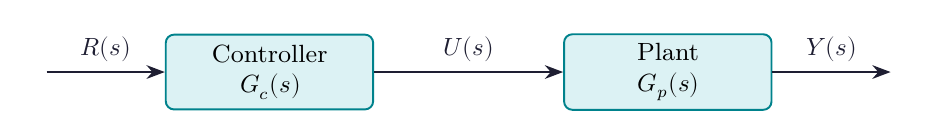
\begin{tikzpicture}[node distance=1.6cm and 2.2cm]
  \node[block] (ctrl) {Controller\\$G_c(s)$};
  \node[block, right=2.4cm of ctrl] (plant) {Plant\\$G_p(s)$};
  \node[left=1.5cm of ctrl]  (in)  {};
  \node[right=1.5cm of plant] (out) {};
  \draw[arrow] (in)    -- node[above]{\small $R(s)$} (ctrl);
  \draw[arrow] (ctrl)  -- node[above]{\small $U(s)$} (plant);
  \draw[arrow] (plant) -- node[above]{\small $Y(s)$} (out);
\end{tikzpicture}
\end{tcolorbox}

$$\frac{Y(s)}{R(s)} = G_c(s)\cdot G_p(s)$$

\subsection{Characteristics of Open Loop Systems}

\begin{tabularx}{\linewidth}{|B{3.2cm}|X|}
\hline
\rowcolor{hdrred}
\multicolumn{1}{|>{\centering\arraybackslash}p{3.2cm}|}{\textbf{\color{myred}Feature}} &
\multicolumn{1}{>{\centering\arraybackslash}X|}{\textbf{\color{myred}Open Loop Behaviour}} \\
\hline
Accuracy          & Low — errors from disturbances or parameter changes are not corrected. \\
\hline
\rowcolor{rowalt}
Stability         & Generally stable; no feedback loop to introduce phase shift or oscillation. \\
\hline
Complexity        & Simple design; fewer components; easy to maintain. \\
\hline
\rowcolor{rowalt}
Cost              & Lower — no sensors, feedback elements, or comparators needed. \\
\hline
Disturbance       & Output permanently affected; no self-correction mechanism. \\
\hline
\rowcolor{rowalt}
Calibration       & Must be re-calibrated frequently to maintain accuracy. \\
\hline
Real Examples     & Washing machine (timed cycle), traffic signal timer, electric toaster, stepper motor. \\
\hline
\end{tabularx}

%═══════════════════════════════════════════════════════════════════════════════
\section{Closed Loop (Feedback) Control System}
%═══════════════════════════════════════════════════════════════════════════════

A closed loop system \textbf{continuously monitors the output} and uses the measured value to correct the control action. The difference between reference and actual output is the \textbf{error}, which drives the controller.

\begin{tcolorbox}[defbox]
\textbf{Definition:} A \textbf{closed loop (feedback) control system} is one in which the output is measured, compared with the reference input, and the resulting \textit{error signal} is used to reduce the deviation. Feedback is typically \textbf{negative}.
\end{tcolorbox}

\begin{tcolorbox}[tikzbox, title={Closed Loop Block Diagram (Negative Feedback)}]
\centering
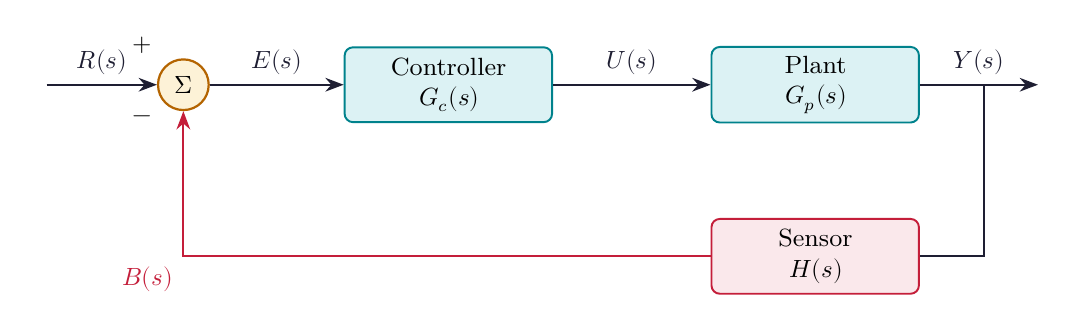
\begin{tikzpicture}[node distance=1.3cm and 1.9cm]
  \node[sumjunc] (sum) {$\Sigma$};
  \node[block, right=1.7cm of sum] (gc)  {Controller\\$G_c(s)$};
  \node[block, right=2.0cm of gc]  (gp)  {Plant\\$G_p(s)$};
  \node[redblock, below=1.2cm of gp](H)  {Sensor\\$H(s)$};
  \node[left=1.4cm of sum]  (ref) {};
  \node[right=1.5cm of gp]  (out) {};
  \draw[arrow]    (ref) -- node[above]{\small $R(s)$}   (sum);
  \draw[arrow]    (sum) -- node[above]{\small $E(s)$}   (gc);
  \draw[arrow]    (gc)  -- node[above]{\small $U(s)$}   (gp);
  \draw[arrow]    (gp)  -- node[above]{\small $Y(s)$}   (out);
  \coordinate (tap) at ($(gp.east)!0.5!(out)$);
  \draw[line]     (tap) |- (H.east);
  \draw[redarrow] (H.west) -| node[below left]{\small $B(s)$} (sum.south);
  \node[above left=1pt and 1pt of sum]{\small $+$};
  \node[below left=1pt and 1pt of sum]{\small $-$};
\end{tikzpicture}
\end{tcolorbox}

\subsection{Closed Loop Transfer Function (CLTF)}

\textbf{Derivation (Unity Feedback, $H(s)=1$):}
\begin{align*}
E(s) &= R(s) - Y(s) \\
Y(s) &= G(s)\cdot E(s) = G(s)\bigl[R(s) - Y(s)\bigr] \\
Y(s)\bigl[1 + G(s)\bigr] &= G(s)\cdot R(s)
\end{align*}

\begin{tcolorbox}[formulabox]
\textbf{Unity Feedback} $\bigl(H(s)=1\bigr)$:
$$\frac{Y(s)}{R(s)} = \frac{G(s)}{1 + G(s)}$$
\textbf{Non-Unity Feedback} $\bigl(H(s)\neq 1\bigr)$:
$$\frac{Y(s)}{R(s)} = \frac{G(s)}{1 + G(s)\,H(s)}, \qquad G(s) = G_c(s)\cdot G_p(s)$$
$G(s)H(s)$ = \textbf{open loop transfer function} (OLTF). \quad $1 + G(s)H(s) = 0$ = \textbf{characteristic equation}.
\end{tcolorbox}

\subsection{Open Loop vs.\ Closed Loop — Comparison}

\begin{tabularx}{\linewidth}{|B{3.0cm}|X|X|}
\hline
\rowcolor{hdrgray}
\multicolumn{1}{|>{\centering\arraybackslash}p{3.0cm}|}{\textbf{Parameter}} &
\multicolumn{1}{>{\centering\arraybackslash}X|}{\textbf{\color{myamber}Open Loop}} &
\multicolumn{1}{>{\centering\arraybackslash}X|}{\textbf{\color{mygreen}Closed Loop}} \\
\hline
Feedback            & Absent                        & Present (negative) \\
\hline
\rowcolor{rowalt}
Accuracy            & Lower                         & Higher \\
\hline
Stability           & More stable                   & May become unstable \\
\hline
\rowcolor{rowalt}
Disturbance effect  & High; no correction           & Reduced; self-correcting \\
\hline
Bandwidth           & Narrow                        & Wider \\
\hline
\rowcolor{rowalt}
Sensitivity         & High to parameter changes     & Reduced (robust) \\
\hline
Cost \& Complexity  & Low                           & Higher \\
\hline
\rowcolor{rowalt}
Real Examples       & Toaster, timer, stepper motor & Thermostat, servo drive, auto-pilot \\
\hline
\end{tabularx}

%═══════════════════════════════════════════════════════════════════════════════
\section{Block Diagram Reduction}
%═══════════════════════════════════════════════════════════════════════════════

A \textbf{block diagram} is a pictorial representation of a control system. For complex multi-loop systems, \textbf{algebraic reduction rules} simplify the diagram step-by-step until a single overall TF $Y(s)/R(s)$ is obtained.

\textbf{Summing junction:} Circle with $+/-$ signs; algebraically adds/subtracts incoming signals.\\
\textbf{Takeoff point:} Node from which the same signal is distributed to multiple branches unchanged.

\subsection{Reduction Rules}

\begin{tabularx}{\linewidth}{|B{3.5cm}|X|C{3.0cm}|}
\hline
\rowcolor{hdrteal}
\multicolumn{1}{|>{\centering\arraybackslash}p{3.5cm}|}{\textbf{\color{myteal}Operation}} &
\multicolumn{1}{>{\centering\arraybackslash}X|}{\textbf{\color{myteal}Description}} &
\multicolumn{1}{>{\centering\arraybackslash}p{3.0cm}|}{\textbf{\color{myteal}Equivalent TF}} \\
\hline
Blocks in Series       & Output of $G_1$ feeds input of $G_2$; same signal chain       & $G_1(s)\cdot G_2(s)$ \\
\hline
\rowcolor{rowalt}
Blocks in Parallel     & Same input, individual outputs summed at a junction           & $G_1(s) + G_2(s)$ \\
\hline
Feedback Loop          & Forward path $G$, feedback path $H$ (negative feedback)      & $\dfrac{G}{1+GH}$ \\
\hline
\rowcolor{rowalt}
Summing pt.\ forward   & Shift summing junction past block $G$ to the right            & Divide shifted branch by $G$ \\
\hline
Summing pt.\ backward  & Shift summing junction past block $G$ to the left             & Multiply shifted branch by $G$ \\
\hline
\rowcolor{rowalt}
Takeoff pt.\ forward   & Shift takeoff past block $G$ to the right                    & Multiply branch by $G$ \\
\hline
Takeoff pt.\ backward  & Shift takeoff past block $G$ to the left                     & Divide branch by $G$ \\
\hline
\end{tabularx}

\subsection{Reduction Procedure (Step-by-Step)}

\begin{enumerate}[label=\textbf{Step \arabic*:}, leftmargin=2.5cm, itemsep=4pt]
  \item Identify and combine all \textbf{cascade (series)} blocks into a single block.
  \item Identify and combine all \textbf{parallel} paths into a single block.
  \item Eliminate all \textbf{feedback loops} using $G/(1 \pm GH)$.
  \item If needed, \textbf{shift} summing junctions or takeoff points to untangle crossed paths.
  \item Repeat steps 1–4 until only a \textbf{single block} $Y(s)/R(s)$ remains.
\end{enumerate}

\begin{tcolorbox}[exambox, title={Exam Tip}]
Always maintain the correct sign ($+/-$) at every summing junction while shifting. Careless sign errors are the most common mistake in block diagram problems.
\end{tcolorbox}

%═══════════════════════════════════════════════════════════════════════════════
\section{Signal Flow Graph (SFG) Analysis}
%═══════════════════════════════════════════════════════════════════════════════

A Signal Flow Graph is an alternative graphical method to represent and solve linear algebraic equations describing a control system. Unlike block diagrams — which require step-by-step reduction — an SFG is solved \textit{directly} using \textbf{Mason's Gain Formula} in a single pass.

\begin{tcolorbox}[masonbox]
\textbf{Definition:} A \textbf{Signal Flow Graph (SFG)} is a directed graph of \textit{nodes} (signals/variables) connected by \textit{directed branches} (carrying gain/transmittance values). It is a compact representation of the system's simultaneous equations.
\end{tcolorbox}

\subsection{Basic Terminology}

\begin{tabularx}{\linewidth}{|B{3.6cm}|X|}
\hline
\rowcolor{hdrpurple}
\multicolumn{1}{|>{\centering\arraybackslash}p{3.6cm}|}{\textbf{\color{mypurple}Term}} &
\multicolumn{1}{>{\centering\arraybackslash}X|}{\textbf{\color{mypurple}Meaning / Definition}} \\
\hline
Node                    & Represents a signal or variable in the system (shown as a small circle). \\
\hline
\rowcolor{rowalt}
Branch                  & Directed arrow between two nodes; labelled with the \textit{transmittance} (gain). \\
\hline
Source Node             & Input node — has \textbf{only outgoing} branches; no incoming branches. \\
\hline
\rowcolor{rowalt}
Sink Node               & Output node — has \textbf{only incoming} branches; no outgoing branches. \\
\hline
Mixed Node              & A node with both incoming and outgoing branches (intermediate variable). \\
\hline
\rowcolor{rowalt}
Forward Path            & Continuous directed path from source to sink in which \textbf{no node is visited more than once}. \\
\hline
Forward Path Gain $P_k$ & Product of all branch gains along the $k$-th forward path. \\
\hline
\rowcolor{rowalt}
Loop                    & Closed directed path beginning and ending at the same node, \textbf{no node repeated}. \\
\hline
Loop Gain $L_i$         & Product of all branch gains around the $i$-th loop. \\
\hline
\rowcolor{rowalt}
Non-Touching Loops      & Two or more loops that do \textbf{not share any common node}. \\
\hline
\end{tabularx}

\subsection{Mason's Gain Formula}

\begin{tcolorbox}[masonbox]
\centering
$\displaystyle T \;=\; \frac{Y(s)}{R(s)} \;=\; \frac{\displaystyle\sum_{k=1}^{N} P_k\,\Delta_k}{\Delta}$
\end{tcolorbox}

\begin{tabularx}{\linewidth}{|B{2.8cm}|X|}
\hline
\rowcolor{hdrpurple}
\multicolumn{1}{|>{\centering\arraybackslash}p{2.8cm}|}{\textbf{\color{mypurple}Symbol}} &
\multicolumn{1}{>{\centering\arraybackslash}X|}{\textbf{\color{mypurple}Definition}} \\
\hline
$N$              & Total number of forward paths from source to sink. \\
\hline
\rowcolor{rowalt}
$P_k$            & Gain of the $k$-th forward path (product of branch gains along that path). \\
\hline
$\Delta$         & Graph determinant $= 1 - \sum_i L_i + \sum_{i,j} L_iL_j - \sum_{i,j,k} L_iL_jL_k + \cdots$ \\
\hline
\rowcolor{rowalt}
$\sum L_i$       & Sum of gains of \textbf{all individual loops} in the graph. \\
\hline
$\sum L_iL_j$    & Sum of gain-products of all \textbf{pairs of non-touching loops}. \\
\hline
\rowcolor{rowalt}
$\sum L_iL_jL_k$ & Sum of gain-products of all \textbf{triplets of mutually non-touching loops}. \\
\hline
$\Delta_k$       & \textbf{Cofactor} of the $k$-th path: value of $\Delta$ after removing all loops that \textit{touch} forward path $k$. \\
\hline
\end{tabularx}

\subsection{Steps to Apply Mason's Formula}

\begin{enumerate}[label=\textbf{\arabic*.}, leftmargin=*, itemsep=4pt]
  \item \textbf{Identify forward paths:} Trace every path from source to sink (no repeated nodes). Note gain $P_k$ of each.
  \item \textbf{Identify all loops:} Find every closed path. Compute loop gain $L_i$ for each.
  \item \textbf{Find non-touching loop combinations:} Identify all pairs, triplets, etc.\ sharing no common node.
  \item \textbf{Compute graph determinant:} $\Delta = 1 - \sum L_i + \sum L_iL_j - \sum L_iL_jL_k + \cdots$
  \item \textbf{Compute cofactor $\Delta_k$:} For each forward path $k$, remove all loops touching that path from $\Delta$.
  \item \textbf{Apply Mason's formula:} $T = \dfrac{\sum P_k\Delta_k}{\Delta}$.
\end{enumerate}

\subsection{Worked Example — Simple Feedback System}

\begin{tcolorbox}[tikzbox, title={SFG Representation}]
\centering
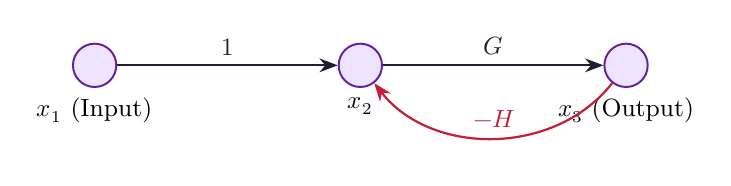
\begin{tikzpicture}[node distance=2.8cm]
  \node[snode, label=below:{\small $x_1$ (Input)}]  (r) {};
  \node[snode, right=of r, label=below:{\small $x_2$}] (e) {};
  \node[snode, right=of e, label=below:{\small $x_3$ (Output)}] (y) {};
  \draw[arrow]             (r) -- node[above]{\small $1$}   (e);
  \draw[arrow]             (e) -- node[above]{\small $G$}   (y);
  \draw[arrow,color=myred] (y) to[bend left=52] node[above]{\small $-H$} (e);
\end{tikzpicture}
\end{tcolorbox}

\textbf{Applying Mason's formula:}
\begin{itemize}[leftmargin=*, itemsep=2pt]
  \item Forward path: $P_1 = 1 \times G = G$
  \item Loop: $L_1 = G \times (-H) = -GH$
  \item No non-touching loop pairs (only one loop).
  \item $\Delta = 1 - L_1 = 1 - (-GH) = 1 + GH$
  \item $\Delta_1 = 1$ \quad (loop $L_1$ touches forward path $P_1$, so removed from $\Delta$)
\end{itemize}

\begin{tcolorbox}[formulabox]
$$T = \frac{P_1\,\Delta_1}{\Delta} = \frac{G \cdot 1}{1 + GH} = \frac{G}{1 + GH} \quad \checkmark$$
Matches the CLTF from block diagram reduction — both methods are equivalent.
\end{tcolorbox}

\subsection{SFG vs.\ Block Diagram — Comparison}

\begin{tabularx}{\linewidth}{|B{3.4cm}|X|X|}
\hline
\rowcolor{hdrgray}
\multicolumn{1}{|>{\centering\arraybackslash}p{3.4cm}|}{\textbf{Aspect}} &
\multicolumn{1}{>{\centering\arraybackslash}X|}{\textbf{\color{myteal}Block Diagram}} &
\multicolumn{1}{>{\centering\arraybackslash}X|}{\textbf{\color{mypurple}Signal Flow Graph}} \\
\hline
Representation   & Blocks, summing junctions, takeoff points             & Directed nodes and weighted branches \\
\hline
\rowcolor{rowalt}
Reduction Method & Step-by-step algebra; multiple passes                 & Mason's formula — single direct computation \\
\hline
Complex Systems  & Tedious; can become cluttered and error-prone          & Compact, systematic, less error-prone \\
\hline
\rowcolor{rowalt}
Gain Formula     & No direct formula; reduce iteratively                 & $T = \sum P_k\Delta_k / \Delta$ \\
\hline
Preferred For    & Simple systems; visual understanding                  & Multi-loop systems; quick TF computation \\
\hline
\end{tabularx}

%═══════════════════════════════════════════════════════════════════════════════
% QUICK REVISION PAGE
%═══════════════════════════════════════════════════════════════════════════════
\newpage
\begin{center}
  {\large\bfseries\color{myred} Quick Revision — Module 1}\\[3pt]
  {\small\color{mydark} Control System $|$ EC601}
\end{center}
\noindent{\color{myred}\rule{\linewidth}{1.2pt}}
\vspace{4pt}

\begin{tcolorbox}[formulabox, title={\textbf{Key Formulas at a Glance}}]
\begin{tabularx}{\linewidth}{B{4.5cm} X}
Transfer Function       & $G(s) = Y(s)/U(s)$ \quad (zero initial conditions) \\[2pt]
CLTF (Unity feedback)   & $T(s) = G(s)/[1+G(s)]$ \\[2pt]
CLTF (Non-unity)        & $T(s) = G(s)/[1+G(s)H(s)]$ \\[2pt]
Characteristic Equation & $1 + G(s)H(s) = 0$ \\[2pt]
Series blocks           & $G_{eq} = G_1 \cdot G_2$ \\[2pt]
Parallel blocks         & $G_{eq} = G_1 + G_2$ \\[2pt]
Feedback reduction      & $G_{eq} = G/(1 \pm GH)$ \\[2pt]
Mason's Gain Formula    & $T = \dfrac{\sum_k P_k\Delta_k}{\Delta}$ \\[2pt]
Graph Determinant       & $\Delta = 1 - \sum L_i + \sum L_iL_j - \cdots$
\end{tabularx}
\end{tcolorbox}

\vspace{6pt}

\begin{tcolorbox}[defbox, title={\textbf{One-Line Definitions}}]
\begin{itemize}[leftmargin=*, itemsep=3pt, topsep=0pt]
  \item \textbf{Control System:} Interconnection of components to regulate output to a desired value.
  \item \textbf{Transfer Function:} Ratio of Laplace output to Laplace input at zero initial conditions.
  \item \textbf{Poles:} Roots of denominator of $G(s)$ — determine stability and transient response.
  \item \textbf{Zeros:} Roots of numerator of $G(s)$ — affect frequency response shape.
  \item \textbf{Open Loop:} Control action independent of output; no self-correction.
  \item \textbf{Closed Loop:} Output fed back and compared with reference; error drives controller.
  \item \textbf{Error Signal:} $E(s) = R(s) - B(s)$; difference between reference and feedback.
  \item \textbf{SFG:} Directed graph of nodes and branches representing system equations.
  \item \textbf{Forward Path:} Path from source to sink with no repeated nodes.
  \item \textbf{Loop Gain:} Product of all branch gains around a closed loop.
  \item \textbf{Cofactor $\Delta_k$:} Graph determinant $\Delta$ with all loops touching path $k$ removed.
\end{itemize}
\end{tcolorbox}

\vspace{6pt}

\begin{tcolorbox}[exambox, title={\textbf{Frequently Asked / Viva Points}}]
\begin{enumerate}[leftmargin=*, topsep=0pt, label=\textbf{Q\arabic*.}, itemsep=8pt]
  \item \Q{Why are initial conditions zero in TF?} TF is an input-output model; it characterises the system, not a specific response. Zero I.C.\ ensures the TF is a property of the system alone.
  \item \Q{What is the order of a system?} Highest power of $s$ in the denominator of $G(s)$.
  \item \Q{Difference between open loop and closed loop?} Open loop: no feedback, no self-correction. Closed loop: feedback present, error-driven, self-correcting.
  \item \Q{What is the characteristic equation?} $1 + G(s)H(s) = 0$. Its roots (poles of CLTF) determine stability.
  \item \Q{When is a system proper?} When degree of denominator $\geq$ degree of numerator ($n \geq m$).
  \item \Q{What is a takeoff point?} A node from which the same signal branches to multiple paths without change.
  \item \Q{What is $\Delta_k$ in Mason's formula?} Cofactor of the $k$-th forward path — $\Delta$ computed after removing all loops that touch path $k$.
  \item \Q{Can SFG and block diagram give different results?} No — both are equivalent representations; Mason's formula gives the same TF as block diagram reduction.
  \item \Q{What are non-touching loops?} Loops that share no common node. Their gain products appear in $\Delta$.
  \item \Q{Why is negative feedback preferred?} It reduces error, improves accuracy, reduces sensitivity to parameter variations, and widens bandwidth.
\end{enumerate}
\end{tcolorbox}

\vspace{6pt}

\begin{tcolorbox}[tikzbox, title={\textbf{Comparison Snapshot}}]
\begin{tabularx}{\linewidth}{|B{3.2cm}|X|X|}
\hline
\rowcolor{hdrgray}
\multicolumn{1}{|>{\centering\arraybackslash}p{3.2cm}|}{\textbf{Property}} &
\multicolumn{1}{>{\centering\arraybackslash}X|}{\textbf{\color{myamber}Open Loop}} &
\multicolumn{1}{>{\centering\arraybackslash}X|}{\textbf{\color{mygreen}Closed Loop}} \\
\hline
Feedback        & No            & Yes (negative) \\
\hline
\rowcolor{rowalt}
Accuracy        & Low           & High \\
\hline
Stability       & More stable   & Can oscillate \\
\hline
\rowcolor{rowalt}
Cost            & Low           & High \\
\hline
Disturbance     & Not corrected & Self-corrected \\
\hline
\end{tabularx}
\end{tcolorbox}

\end{document}
